

%%%%%%%%%%%%%%%%%%%%%%%%%%%%%%

% NICE EXPLANATION TO USE SOMEWHERE

% The need for fast, complex, and responsive AJAX-powered Web applications demands replication of a lot of this logic on the client side, dramatically increasing the size and complexity of the code residing there. Eventually this has brought us to the point where we need MVC (or a similar architecture) implemented on the client side to better structure the code and make it easier to maintain and further extend during the application life-cycle.

%%%%%%%%%%%%%%%%%%%%%%%%%%%%%%

\chapter {Design Alternatives for Modern Web Applications}
\section{Introduction}
So far we have discussed the behavioral trends in modern Web applications and the technologies that runs them. We saw that modern Web applications are often very interactive with rich user interfaces, that looks and performs like native desktop applications with graphical user interfaces. In this chapter we look at popular ways these applications are built. This concerns the application's \textbf{architecture}, which is a concept that describes the application's structure, at different granularities. 

The traditional Web application has in the last decade followed a thin-client approach where all the logic happens on the back-end. In such architectures, HTML pages are dynamically generated on the server and handed to the browser every time the client issues an HTTP request. Lately however, there has been an increasing interest in moving much of the application's logic to the client, and abandoning the server-side page generation in favor for client-side page generation. This is called a thick-client architecture.\footnote{The thick-client architecture is not a new idea; thick-client architectures have been around for many years, where programs are sent from the server and executed on the client. Often this would be online games, calculators, or other user-interactive applications. However, these applications depend on a specific program that is compiled and executed on the client, in other words, not traditional Web pages that uses common browser-supported technologies.} Still however, a lot of applications follow the traditional approach, as many developers and application owners are skeptical to the thick-client model; this architecture implies heavy use of JavaScript, which has since its beginning had a lot of opposition, and people are still using old browsers that does not fully support JavaScript\cite{ie6use}.

The main purpose of this chapter is to outline the differences between, and popular ways to build traditional thin-client architectures, and innovative thick-client architectures. This also includes popular database solutions for persisting data in Web-apps. The first part of this chapter is divided into two main sections, one for each architecture. After this we will see how these concepts have been used in the prototypes built for this thesis. We will refer to the traditional approach as \textbf{Reference-model 1.0}, while the latter approach will be referred to as \textbf{Reference-model 2.0}. Thus, these two will be our reference models for software architectures that are aimed to build modern, interactive and scalable Web apps. 

\section{Reference-model 1.0}
Going back approximately 15 years, dynamic Web applications where often built with Common Gateway Interface (CGI) technologies\cite{cgi}. With CGI, a Web server accepts URLs that are delegated to an appropriate back-end program. A process is started on the server, and the CGI program executes the given request, which results in an HTML page that is sent back to the client. This solution however, was not very scalable considering each request would trigger a new process on the server. Gradually, as the Web got more users and the applications became more complex, new Web framework technologies came along. Examples are PHP\cite{php}, Java EE\cite{j2eeglance}, Ruby on Rails\cite{rails} and Microsoft's .NET\cite{popFrameworks}. For many years, developers have been building Web applications with these technologies, where all of the application's logic is executed on the server. This implies that the back-end implementation has many responsibilities, and the front-end is simply a thin-client that doesn't need to do much processing. This is only logical, as back-end implementations run on powerful Web servers, and client devices has up until recent years not been able to perform demanding processing jobs.
	
\subsection{The Three-Layered Architecture}		
A classical way of separating concerns in a Web application is to divide the whole system into three different software layers. There are some variations to how these layers are separated, but in this thesis, when we refer to a three-layered architecture, we follow the layering structure outlined by Brown et al\cite{brown}. This architecture separates the system into a presentation layer, domain logic layer, and a data source layer. The layers reside exclusively on the back-end of the application. The front-end has little responsibility in this architecture, as its only task is to display the result that is produced on the back-end. The layers are designed to be very loose-coupled. This is done by avoiding that a module in one layer depends on a concrete implementation in a lower layer. Instead, they depend on abstractions (interfaces) which can easily be swapped out. This principle is often referred to as the dependency inversion principle \cite{dipioc}. The abstractions are not hard-coded into the layers, but are "injected" through function arguments so that the same function can be called again if one wants to change the type of a dependency. The benefits from having individual implementation details encapsulated in different layers, is that it is very easy to modify one layer without harming another, and components can easily be reused. This facilitates a flexible and maintainable codebase\cite{flexible}.
		
\paragraph{The Presentation Layer} is the application's main entry point. Each URL offered by the application is mapped to a dedicated handler (often called a \textbf{controller}) in the presentation layer. In modern Web apps, the presentation layer is often implemented with the \textbf{Model-View-Controller} pattern\cite{mvc}. This is an architectural design pattern that organizes the structure of the layer. In this pattern, \textbf{controllers} handle HTTP requests from the client and simply delegates to a proper business operation in a lower layer. The result from the business function is returned in terms of \textbf{model} objects, which implement the \textbf{domain} of the application. When a business function returns the controller, it looks at the result to determine which \textbf{view} to return back to the end user. The view might be an HTML page, an HTML template file, or another data-format like XML or JSON. The latter two formats are most often used if the request is an AJAX request. If it is a template file, the view is sent to a rendering engine before the resulting HTML is returned to the client. Often, template files have references to other template files, in which case these will be merged together by the rendering engine. This facilitates decoupled view logic with fine-grained templates that can be reused.

Another architectural structure is the \textbf{Application controller pattern}\cite[p.379-386]{poea}. This separates how objects are to be presented in the app, from the app's business operations, by adding a new layer which is responsible for deciding which page to show in which order. This structure is nice if there is a lot of logic required to decide the page's ordering and navigation scheme. However, as the most common architectural pattern for the presentation layer is with the MVC pattern, we will continue the discussion with this pattern in mind. 

When a URL request comes in through the presentation layer, it might go through a number of \textbf{filters} before control is handed to the controller. Filters can have different objectives like authentication, marshalling of different Web formats into an object in the programming language that is used, error handling or HTML form validation. Also, the presentation layer would check the URL for a session identifier in the request's cookie, or the Url itself. The session identifier is referencing a session object that is already residing on the server's main memory, or in a database. The session object can also be used to store state information for the User, and to hold authentication details. After the request has passed the filters, the appropriate controller handler is called, which delegates control to a business function, typically in the domain logic layer. 


\paragraph{The Domain Logic Layer}, also called the business logic layer, or service layer, is responsible for executing the business operations that are supported in the Web application. These are the functions that makes up the core services of the application. Like in the presentation layer, the domain logic layer operates on the domain objects (i.e models). The business operations in the domain logic layer uses the domain objects by executing operations on them. Examples are calculating the total price for an order of books, registering a new friendship between two users, or searching for recommended movies for a currently logged in user. The domain logic layer sends and receives domain objects from the data source layer in order to persist them in a database. 

There are multiple ways of organizing how the business processes are implemented in the domain logic layer. A simple structure is by using the Transaction Script design pattern \cite{poea}. In this structure, each business operation is implemented in a single self-contained and independent procedure (script). Each procedure is mapped to an operation in the presentation layer, that takes input from the presentation layer, performs business logic (e.g data validation, calculations etc) and stores data in the database. This approach is very simple, as there is no domain abstraction and complex object-structure, just independent functions. However as applications get complex this pattern might lead to code duplication as different transactions might have common behavior. Another more common and object-oriented structure is to use the \textbf{Domain Model design pattern} \cite{poea} where business logic is encapsulated in domain objects. For example a BookOrder class would have functions for creating a book order given a list of books and a user id, fetching a book order given an order Id, updating a book order, and deleting a book order. In addition, the domain objects encapsulate the data attributes that represent the state of the object. The domain objects can have dependencies on each other, and call each others function in order to gain code reuse.
	
\paragraph{The data source layer} is responsible for communicating with other systems, such as databases, messaging systems, external Web services, the filesystem etc. Traditional Web architectures uses a relational database management system, which is the most popular solution for choosing how to persist the data in modern Web-apps\cite{dbpop}. Thus our Reference-model 1.0 will define that data is persisted in a relational database. The reason for its popularity is much due to the relational model, which brings a flexible and highly efficient query language (SQL). Most computer science courses on databases teach SQL, so developers tend to think data relationally. Also, data safety guarantees are provided with ACID, and the wide offerings of relational database management systems with its many development toolkits makes it a natural choice. Not to mention, the technology itself is many decades old and therefore brings years of experience and documented best-practices. 

The data source layer is responsible for marshalling domain objects into proper storage representation (also called database mapping), and vice-versa. For instance translating a SQL table into a Java object. The data source layer has to connect to the database, handle database transactions and close database connections. Usually this is handled by the Web application framework, so the data source layer only has to worry about how to perform operations on the database. As with the domain layer, there are two popular design patterns for structuring the data source layer. One is with the active record pattern \cite{poea}, in which case each domain object would know how to perform CRUD operations on themselves. Another approach is the data mapper pattern \cite{poea} where there is one separate class for each domain object, that performs marshalling of the given domain object, and is responsible for implementing CRUD operations on behalf of its domain object. The data mapper pattern separates the persistence code out of the domain objects, but adds more classes to the system. The active record pattern has a tendency to grow big in size, if the domain objects has to support a large amount of complex database operations. 
	
There are also frameworks that perform the marshalling, given some simple configuration of the domain objects. These are called object-relational mapping (ORM) tools. They often provide caching mechanisms to avoid using the database as much as possible, and they allow the programmer not to worry about marshalling at all. In many cases this could lead to less code in the data source layer. \cite{tedorm} Examples are Hibernate \cite{hibernate} for java, MyBatis\cite{mybatis} for Microsoft .NET and Java, and LINQ \cite{linq} for Microsoft's .NET. It is important to point out that even though these frameworks hide the complexity of object-relational mapping, it does have some pitfalls. Many developers argue that by using ORM-tools you loose the ability to exploit the full features of a database management system\cite[p. ~124]{ormlame}. This includes the ability to do customized database tuning, and take advantage of special data types that are supported by specific vendors. Plus, the fact that an ORM-tool does indeed hide the object-relational mapping code, makes it harder to debug, and also, there might be some performance overhead due to the complex code that is generated by the ORM framework.	
	
\subsection{The Front-End}
Up until now, we have been discussing the back-end implementation of a traditional Web app. The front-end consists of the set of HTML pages, CSS style sheets and JavaScript files that makes up the user interface of the application. User-navigation in traditional Web apps is often done through HTML forms or hyperlinks, which leads to a new page that is completely rendered on the browser (a page refresh). 

Also, in cases where a highly interactive event is to happen, a dedicated JavaScript event handler that is registered to listen to certain events will perform the action. This could be displaying a pop-up window or an animation effect on a mouse-hover event. The event handlers are registered with the browser when the HTML page is first rendered. In traditional Web apps, these handlers are often self-contained and independent JavaScript functions that has no structure or modularity. In most cases, this is because of some developer's relaxed relationship to the language; the JavaScript code is developed by adding function after function that merely serves to implement a new dynamic feature. This often leads to spaghetti code\cite{spagetticode}, in cases for applications that include a lot of interactive JavaScript behavior\cite{spagethi}.
				
\subsection{Platform Environment}
Another aspect of the classical three-layered architecture is application tiering.\footnote{Application layering is a term that divides the code into separate logical software layers. Application tiering on the other hand, is another logical separation often associated with where these "tiers" are physically deployed. For instance a three-tiered Web application could have its presentation tier on the Web server, the logical tier on a dedicated application server, and the persistence tier on a dedicated database server.} A Web application is often divided into three tiers; the presentation tier, the logic tier, and the persistence tier. 

The Web server hosts the presentation tier which communicates with client users through HTTP. The Web server listens on port 80, which is the port number used for HTTP. The HTTP request is forwarded directly to the appropriate code on an application server. The application that runs on the application server communicates with the persistence tier that is usually hosted on one or more database servers. In a bigger production environment, it is normal to distribute the tiers into separate physical server machines (called horizontal scaling). Each server is hosted on a separate machine in a so-called \textbf{shared nothing} manner, meaning the servers on each tier are independent so they don't have to communicate with each other. This makes it easy to add more servers on demand without any synchronization difficulties. Note that when the persistence tier is composed of a relational database management system, a shared-nothing architecture is difficult to implement, due to the nature of the relational model \cite{cloudmanagement}. This makes it difficult to do horizontal scaling with relational database systems. 

However, some SQL systems are particularly designed to scale vertically\cite{sqlscale}, and many large-scale Web 2.0 applications does successfully implement shared-nothing architectures backed by multiple distributed SQL databases. One example is the social-networking site Pinterest\cite{pinterest}. A report\cite{scalepint} outlined their platform environment, which among others include:
\begin{itemize}
\item{} 88 MySQL servers
\item{} 180 Web servers
\item{} 240 Application servers
\item{} 200 cache servers
\end{itemize}
				
\subsection{Examples of traditional Web architectures}
In this section we look at two examples of some common, traditional three-layered Web application architectures. The examples use Web application frameworks that is made for different programming languages, and promotes different architectural solutions. The purpose is to propose a set of popular Web architectures, that will be used as a base to determine the architecture we use to design the first prototype in this project. 
				
\paragraph{MVC with Ruby on Rails}. The Rails framework for Ruby has become a highly popular backend technology for Web applications, having many big commercial users. The framework is built around the MVC design pattern \cite{mvc}. In a Rails application, the controllers act as thin classes that receives a URL request, and  delegates business logic to the models. A model is a Ruby class that implements the Domain Model design pattern. The views consist of HTML template files, often written in a template language like HAML\cite{haml} or Mustache\cite{mustache}. These templates can reference data variables in a model class, and are rendered into HTML files on the server before they are sent to the client's browser. 

The data source layer in Rails is typically built with the Active Record design pattern. This works by letting the model objects implement CRUD operations for manipulating the database. This way, every model class contains business logic operations and the functions required to persist and manipulate the particular model in the database.

\paragraph{Front Controller with SpringMVC}
SpringMVC is a Web framework that wraps the Java Servlet API technology. The Java Servlet API is a set of classes that implements low-level protocols to communicate on the Web (e.g HTTP). For example, the Java Servlet API implements an interface called \textit{javax.servlet.http.HttpSession}, which provides session management. This session implementation puts an Id (called the JSESSIONID) in the User's HTTP cookie. This Id refers a particular HttpSession object that belongs to the User, and it is maintained by Spring on the server. 

Just like with Rails, SpringMVC is also built around the MVC pattern. However, the framework also applies an architectural pattern called the Front Controller pattern\cite{frontcont}. This pattern works by having one central servlet (the front controller) that receives all HTTP requests, and delegates control to a set of components that handle the request. This can be seen in figure \vref{fig:springmvc}.
	\begin{figure}
	\begin{center}
	\fbox{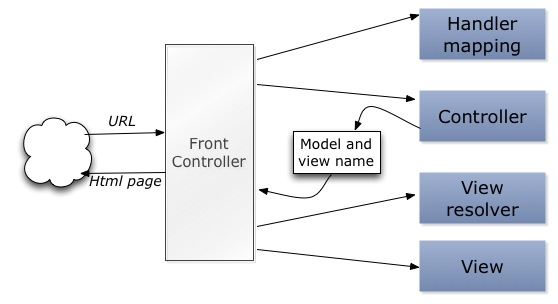
\includegraphics[width=10cm] {images/springmvc.eps}}
	% Kommandoen \fbox tegner en ramme.
	\end{center}
	\caption{A request flow with spring MVC}\label{fig:springmvc}
	\end{figure}
	
When a request comes in, the front controller will ask a \textbf{handler mapper} to get a reference to a specific controller based on information provided in the request URL. A controller is a SpringMVC component (related to the controller in the Model-View-Controller pattern) that is responsible for processing the actual requests. The handler mapper, is another Spring component that in addition to knowing what controller to issue based on a URL, performs pre- and post processing (i.e filtering) procedures, such as HTML form validation. When the handler mapper is finished pre-processing a URL request, it returns a reference to the right controller. The front controller then delegates the request to this controller. The controller typically just delegates to a business operation, and upon completion, it populates a model object with necessary data that is to be displayed in the view. The model object is a simple key-value data structure that lets the developer easily reference its data from the view file. The controller function also returns the name for the view that is to be rendered together with the model object. The view is a template file, often written in a template language such as JSP\cite{jsp} or Velocity\cite{velocity}. It is the view resolver that maps a logical view name (e.g "homePageView") to a physical view name (e.g "/WEB-INF/views/homePageView.JSP"). Finally the view and the model object is rendered to HTML and send back to the client. 
	
With Spring comes a great implementation of an inversion of control container (IOC)\cite {dipioc}. Inversion Of Control is a programming methodology where the concrete types of object references are not known at compile time, because the references are instantiated and populated  by an assembler at run time. This avoids having tight couplings between classes, and promotes a flexible codebase. The IOC container is a module that is responsible for creating objects, populate their references  to other objects, and manage their complete lifecycle. The container is fully configurable, which makes it easy to decide how the classes are instantiated. For example, objects can be configured to be lazily instantiated, meaning the object won't be instantiated until it is first referenced. Also, there are multiple ways Spring's IOC container can be configured to create objects. In Spring, this is referred to as the object's \textbf{scope}. Some common scope-alternative are:

\begin{itemize}
\item{} Request - one instance is created for each HTTP request
\item{} Session - one instance is created for each HTTP session
\item{} Singleton - only one instance of the given class is ever created.
\end{itemize}
			
A typical domain logic layer in a Spring application is built with the service layer pattern \cite{serviceLayer}. In the service layer pattern, the business logic is split into two. A service layer that exposes an API that encapsulates all the business operations, and the domain model which encapsulates the application's domain in separate classes that merely keeps data variables. The API, or service layer is categorized into logical abstractions called \textbf{services}, where each abstraction is hidden behind a facade \cite[p. ~158]{facade}. A facade is an interface that contains simple access methods to a more complex set of data structures, like complex business operations or database access methods.  Hence, each service encapsulates complex business operations and communicates with lower layer data source functions. The domain objects typically has no logical functions, only private data attributes with accessor methods, as opposed to the domain model design pattern. The service classes are also responsible for handling transaction management, so that if a transaction fails, the service classes know how to handle it. When performing database transactions, the service classes delegates to the data source layer which would know how to communicate with the database and perform object-relational mapping. This could be done by implementing a customized object-relation mapping scheme, for instance by implementing the data mapper pattern described earlier, or by using an ORM tool such as Hibernate or JPA\cite{jpa}. The latter case is similar to the active record pattern, often used in Ruby on Rails. Spring is one of the most popular frameworks for Java, as of 29th April 2013\cite{popFrameworks}.

\section{Reference-model 2.0}
The motivation for proposing a reference model for modern Web app architectures has its roots in an architectural shift that started around 2010, when browser's capabilities to execute JavaScript increased tremendously. This was by the time when Google launched its Chrome browser with the powerful V8 JavaScript engine, and the compelling browsers followed along with similar JavaScript capabilities. Also, The JavaScript language itself has started to get much more endorsement from the Web community with the standardization of ECMAScript, and Google's provenly working large-scale JavaScript applications like Gmail, Google Maps and also Node.js. This has led to many new experimental Web architectures that takes a distance from the thin-client model, and where application logic is gradually moving from the server and into the client. This means that the back-end is left being a simple and agnostic storage center for persisting the domain data in the application. Not only is this feasibly, but it's becoming increasingly popular. However, many developers have a skeptical relationship to JavaScript, partly because JavaScripts history of buggy features and browser incompatibility problems. Also, many developers are not aware of JavaScript's features like object-orientation including prototypal inheritance, and functional- and dynamic programming facilities, having closures and a dynamic typing system. Instead, they have acknowledged the fact that building large-scale JavaScript applications doesn't scale in terms of code maintainability; it often ended up as piles of spaghetti code\cite{spagethi}. This is an unfortunate misinterpretation. 

Together with this thick-client approach one has also seen a sudden interest in alternatives to the traditional relational database. With the increasing popularity of applications being deployed and run in the cloud, there is a need to be able to distribute an application's database over many servers. Now, because traditional SQL databases has showed not to replicate very easily\cite{cloudmanagement}, this issue, together with a need for a simpler programming interface against the database, has led to the many alternative NoSQL databases. 

In this section we propose an architectural approach where the application is moved to the client using JavaScript, and where data is persisted with NoSQL technologies.

\subsection{Front-end Frameworks}
An interesting aspect of modern Web application development is the evolution of JavaScript development environments. Not only has JavaScript been judged for being a language with many limitations, but it has also lacked proper frameworks and plugins for simplifying development of large-scale applications. However with the increasing interest for such JavaScript applications, a huge amount of frameworks and language variations have been built. This includes:
\begin{itemize}
\item{} Frameworks for structuring and organizing JavaScript code. \footnote{There is an project\cite{todo} on www.Github.com\cite{github} where developers are implementing the same Web application with different JavaScript frameworks to help developers choose a proper code organization framework for their Web apps.}
\item{} Programming languages that compile to JavaScript, to facilitate the development of large-scale JavaScript applications with a language that is more similar to traditional languages like Java or Ruby. Examples are Coffescript\cite{coffe} and Clojure script\cite{clojure}.
\item{} Frameworks for syntactic sugaring of the JavaScript language, useful mathematical operations, fixing browser compatibility issues, and simplifying working with the AJAX technology \cite{serrano2007ajax}. Popular examples are JQuery\cite{jquery}, Dojo\cite{dojo} and Backbone.js\cite{bakbone}.
\item{} Rendering engines for the front-end, built to produce HTML given a template file and data objects.
\end{itemize}

\subsection{Thick-Client Concepts}
Having the application moved to the client means that the one-to-one mappings between user interactions and controller handlers on the server are gone. Instead, these events are now picked up by JavaScript handlers on the front-end. The front-end has taken over many of the concerns that used to be implemented on the server. This includes: 
\begin{itemize}
\item{} Routing between pages
\item{} Render views into HTML
\item{} Sessions and state handling
\item{} Business logic operations
\item{} Deciding what to store in the database and when
\end{itemize}
 
Now, there might be other concerns that can be moved to the client as well, such as language translation of content and third-party API requests. However, I decided that this goes out of scope for this thesis. Also, there are variations in to what extend all of these responsibilities are performed on the client. For example, developers at Airbnb\cite{airbnb} found that they could benefit from letting the server be involved in routing between pages \cite{airbnbnode}. Also, Twitter \cite{twitter} found that letting the server participate in page rendering had good performance benefits\cite{timeToFirstTweet}. However, the main motivations for moving code to the client is because one might achieve:

\begin{itemize}
\item{} Better response-times, because tedious server requests can be avoided 
\item{} Better scalability, because less work has to be done on the server
\end{itemize} 
 
\subsubsection{Moving the Application to the Browser}
In Reference-model 2.0, the application relies on the front-end, and is completely written in JavaScript, or a language that is compiled to JavaScript such as CoffeScript, or ClojureScript. The JavaScript code can either be sent to the client all at once when the Web application is first accessed, or parts can be lazily fetched when needed. This requires the source code to be split into separate code files so they can be sent individually from the server. This might be a performance benefit in case the whole JavaScript codebase is very big. A pitfall however might be that very many small JavaScript files would be required and sent simultaneously, in effect potentially causing tedious transmission times. In some cases the TCP connection overhead might be a performance bottleneck because the browser usually creates a new TCP connection every time the browser requests something from the server. 

	
\subsubsection{Single-page Web Application Architecture}
One essential advantage with the thick-client architecture is that server requests might be limited. In the traditional approach, each user interaction with the page leads to a server request that result in a new page, and the browser has to reload the whole page. This causes a disruption in the user experience. With the modern approach, the request goes straight to JavaScript event handlers. This way, the client stays on the same page during the whole session, requiring no new page reloads. If for instance a link in the navigation bar that leads to a different page in the application is requested, everything is done in the browser by manipulating the DOM tree so that the new page is displayed. This could lead to a much more fluid user experience, because server requests can be avoided, and the browser does not have to reload the entire page. This principle is commonly referred to as a Single-page app\cite{spa-man}.

If the front-end needs to synchronize data with the database it will send an asynchronous data request to the server with AJAX. This could for instance be to save some data, or get some new data that needs to be displayed on the page. The client can also store data in the browser's memory, such that the more domain objects stored in the browser's JavaScript memory heap, the less requests has to be sent to the server. Depending on the application, write, update and delete operations will always sooner or later have to lead to a server request, so that every user has an up-to-date view of the data. In applications that require all updated data to be available as close to real-time as possible, the data has to be directly written to the database, in effect work as a write-through cache. In applications where this requirement is more relaxed, the front-end can choose to perform persistency at a later and more appropriate time. For Web 2.0 applications, the former is often wanted, because users usually want to see the latest updated data at all times. 
		
\subsection{The Simplified Back-end}
The responsibility of the backend is mainly to manage the database. It's interface is still exposed as controller handlers, however these are not customized for particular HTML form requests or hyperlinks that leads to a new HTML page. Instead, the backend exposes an \textbf{API} for manipulating with the application's domain in the database. This API contains a set of public functions where each function is identified by a specific URL. Each URL refers to a domain entity in the application, and an operation that the server is to perform on the domain object. Note that this operation is usually not a complex business operation, but merely a single database operation. The operations offered by the backend API are commonly expressed using merely HTTP methods. Hence, the server API is a RESTfull service that adheres to the principles in the REST design pattern. Now, instead of creating and returning a complete HTML page upon each client request, the server would return a more fine-grained data object represented in a uniform data format such as XML or JSON. This is a much more general-purpose solution, because external clients like mobile applications and other third party applications can now use the service offered by the application, and so choose how to use and display the returned data.\footnote{A typical service-oriented architecture}

In respect to Reference-model 2.0, the back-end can be implemented using basically every server-side Web application framework, considering the responsibility of the back-end is so very simple. Popular choices are among others Ruby on Rails, SpringMVC and Node.js\cite{popFrameworks}.

\begin{table}
	\centering
	\begin{tabularx}
	{\linewidth}{ |X|X|X| }
	    \hline
	    \textbf{Method} & \textbf{URL}  & \textbf{Description} \\ \hline
	    Get & www.shredhub.com/ shredder/1234 & Get shredder with id 1234 \\ \hline
	    Post & www.shredhub.com/ shredder/ ?name=Jude Swayer & Add shredder with name Jude Swayer  \\ \hline
	    Put & www.shredhub.com/ shredder/ 1234?country=Sweden & Update shredder with id = 1234 set country = Sweden \\ \hline
	    Delete & www.shredhub.com/ shredder/1234 & Delete shredder with id 1234 \\ \hline
	    \end{tabularx}
	    \caption{A simple REST API}
	    \label{table:urls}
	   \end{table}
	   
\subsubsection{REST API's and JSON}
The thick-client model avoids letting the user communicate synchronously with the server. Instead, the JavaScript application that runs in the browser is responsible for knowing when it needs to communicate with the server. This would be whenever some domain objects that are not already in the browser's heap are requested, or some domain object must be persisted to the database. The requests to the server are exclusively done through the RESTful API. This means that all domain objects that are to be offered by the server, must be accessed through one of the HTTP methods \textit{Get, Post, Put, or Delete}. An example of a RESTful API that offers functions for persisting a Shredder object is showed in table \ref{table:urls}. A shredder is a guitarist in the Web app prototype that has been created in this thesis.
	    
	The server would respond with the domain objects in JSON format, instead of a complete HTML file. This way, it is up to the client how to visualize the result-data. Also, the API is very consistent, because it adheres to a common interaction scheme, namely the HTTP request methods Get, Post Put, and Delete. This creates a familiar and easy-to-understand server API. This programming interface works really well with the thick-client model, because the client tier can be completely responsible for maintaining the application's state, and thus the server can be stateless.
	
Modern REST API's very often use JSON as the transmission format, because it fits well into the programming model both on the front-end and back-end, because considering that the front-end code is implemented in JavaScript, and JSON is part of the JavaScript language, it is very appropriate to use JSON as a transmission format because no marshalling has to be done on the client. This might also apply on the back-end: Some NoSQL technologies stores JSON-like objects, in which case no marshalling would be needed if the programming language used supports JSON.
	
\subsection{Modular JavaScript}
A modular codebase is made up of highly decoupled, encapsulated pieces of coherent features that are implemented in separate modules. A codebase that consists of loosely coupled modules, facilities a flexible and maintainable system, because the codebase contains less dependencies\cite{flexible}. This makes it easier to change one part of the system without harming any other.  

The JavaScript programming language does not have module features built into the language. This means that it is up to the developers themselves to develop some sort of module framework. Various design patterns have been proposed to establish standard ways of developing modules, like the module and sandbox pattern \cite{jspatterns}. These are patterns that gathers related code into coherent modules, fairly similar to classes in traditional object-oriented languages. A lot of work has been done to provide open solutions for JavaScript developers to build modular JavaScript code in the browser. A common solution is Asynchronous Module Definition (AMD)\cite{amd}, which is an interface proposal for how to create modules in JavaScript. Having the JavaScript code separated into modules means that these modules can be split into separate source files and have references to each other. That is what facilitates the lazy loading of JavaScript files previously mentioned.
AMD makes it possible for the modules to depend on each other, and also on HTML templates, so that whenever a JavaScript module is fetched from the server, the HTML template will be fetched as well, and will be available as a text string inside the JavaScript module.
	
The AMD principle was also made to have a better alternative to loading scripts then the traditional group of \textit{<script>} tags embedded in HTML files. The problem with this approach is that it doesn't say anything about the loading order, meaning if any of the scripts depend on each other, there is no guarantee they will be fetched in the right order. AMD brings an API that defines all the dependencies for the modules. As such, when a module is needed, all its dependencies are first loaded asynchronously, and when they're all received from the server (or some other external source), the dependencies are made accessible inside the module. The AMD API comes with two functions: \textit{require()} and \textit{define()}. \textit{Define()} is used to encapsulate a JavaScript module, and make it globally accessible, while at the same time define the other modules it depends on. The \textit{require()} is used to asynchronously load modules into a function, in which the function will not be called until all the modules are loaded and ready to be used inside the function.


\subsection{Client-side Page Rendering}
What is special with Reference-model 2.0 is that rendering HTML is no longer a matter of rendering a complete HTML page, but rather render the parts of the HTML page that need to change, and render this immediately without consulting the server. One approach is to write blocks of HTML with JavaScript strings, and write this to the DOM when a page needs to change. However, this is not very clean, or maintainable, especially when building large applications.

Using HTML templates are preferable as these can be reused, are easy to read and can be cached in the browser. Whenever the HTML need to change, a JavaScript rendering engine will be consulted which performs the rendering. The result is either appended to the DOM, or swapped with current DOM elements.

As previously mentioned, the AMD model makes is possible to have JavaScript modules that depend on HTML template files. This facilitates a nice programming model, because if the HTML pages are also separated into small independent templates, then these templates can be stitched together to form complete HTML pages. As such, HTML templates can be reused, removed or swapped out from the current HTML page by the JavaScript renderer. This enables a highly flexible way of altering contents of the HTML page, and efficiently altering large parts of HTML without consulting the server.
		
\subsection{Client State and Navigation Handling}
Another part of Reference-model 2.0 is how the state is being kept between requests. The major goal of Reference-model 2.0 is to move much of the application logic from the server to the client. Thus, being able to keep the state client side is of high priority. In Reference-model 2.0, we propose an alternative solution to this by using HTML 5's Web Storage\cite{webstorage}. The HTML 5 Web storage is a standardization made by W3C that offers a way to store data in the browser between page requests. It is supported in all modern browsers. HTML 5 Web storage contains two storage containers: \textbf{localStorage} and \textbf{sessionStorage}. The difference is that local storage is being persisted even when the browser is closed, and it has no expiration date. The session storage is only kept in the browsers memory until the session is over, which means either if the user closes the tab or the browser. The Web storage enables developers to store lots of more data than what it supported with cookies. As an example, Internet Explorer 8 allows for sessionStorage up to 10 mega bytes, while a cookie is generally limited to 4 kilo bytes. The sessionStorage consists of a key-value data structure that is accessed by a simple JavaScript API.
	
A session implementation can be built by letting a JavaScript object be created when the Web application is first accessed by the client user. The object is populated with user data, and so each time the client tier changes state or receives some state information from the server, it can be persisted in the session object. Thus the server does not have to maintain a session object in memory for each user that is currently logged in to the Web application.

Navigation is done without consulting the server, meaning all User interactions that would normally result in a new page is now picked up by a dedicated JavaScript component. This component is often called a \textbf{router}. The router's job is to ensure a new page will be rendered in the browser (typically by delegating to a proper view-logic implementation), and change the browser's URL to match the new state.\footnote{Changing the browser's URL recently became much simpler with the HTML5 browser history API\cite{html5history}, which enables developers to change the URL with JavaScript.}

\subsection{Alternative Front-end Design Patterns}
There are many ways in which to structure the JavaScript code that runs in the browser. As we did for Reference-model 1.0, we will look at some popular architectural design patterns for structuring front-end code. 
\begin{itemize}
\item{} MVC/MV*: Traditional Web-apps often implements the MVC pattern. In thick-client architectures, this pattern is often used, however with some variations.  Models represent the domain data and communicates with a back-end API, while views contain logic that handles the user interface (\textbf{view logic}). In Reference-model 1.0, view logic was done both in JavaScript handlers on the front-end, and controllers and HTML templates on the back-end. Controllers handle routing between views and models. However, MVC-style controllers in server-centric applications doesn't always transfer directly to the thick client architecture. Controller behavior is often implemented in both views, and the router. Therefore, a popular way to define a thick-client's architectural pattern is simply MV*, meaning models-views- and something else that's up to the developer. 

\item{} MVP: Is a pattern that decouples the views from models by introducing a mediator called the presenter. In this pattern, the view's responsibilities are merely thin containing little to no logic, all of which is done by the presenter. The presenter's responsibility is to handle all presentation logic and routing, and communicate with a persistency layer on behalf of the models. The pattern is mostly used in cases with complex views and many different user interactions, such that handling logic and routing can be separated and reused as much as possible in the presenters.
\item{} MVVM: Is a pattern that adds an abstraction called the view-model. Its responsibility is to turn models into their user interface representation, and delegate commands from views to models. Thus the views don't have to worry about how the models should look like, or how to delegate business logic. The pattern is also suitable when models must have many different view representations.
\end{itemize}

\section{The Solutions Chosen}
The two reference models just described are popular approaches to how developers design and implement modern, interactive Web apps. In this thesis, the goal is to compare these two approaches, in order to identify their strengths and weaknesses.  Therefore, the main concepts from these reference models are applied in two different software architectures for a prototypical Web app. The first solution is called \textbf{Architecture 1.0}, while the latter is called \textbf{Architecture 2.0}. 

Architecture 1.0 is a thin-client application, where the application relies on the back-end. The back-end is built as a three-layered architecture. This means that all the view logic happens in the presentation layer on the server (and some is made with JavaScript on the front-end), business logic operations happens in the domain logic layer, state is being kept on the server using HTTP sessions, and the front-end tier is tightly coupled to the server such that each HTML form or link has a corresponding handler on the server which serves to generate a new HTML page given the result of the request. The back-end is built with Spring MVC, and is therefore a Java Web app. It uses a SQL database to persist data, and does not use any ORM tool to perform database mapping. 

Architecture 2.0 is a thick-client architecture where the application resides on the front-end. State management, controller handling and business logic all happens in the browser, which is built purely with JavaScript. The front-end uses the MV* pattern, where models are active record objects that uses the back-end only as a simple data repository. The back-end is offering its services through a Rest API, which is built with Node.js. The Rest API manipulates the database, which is a MongoDB database. 
			
\begin{table}
\centering
	\begin{tabularx}
	{\linewidth}{ |X|X | }
	    \hline
	    \textbf{Reference-model 1.0} & \textbf{Reference-model 2.0} \\ \hline
	    Server-side page rendering & Client-side page rendering \\ \hline
	    Application logic is on the server (thin-client) & Application logic is in the browser (thick-client)  \\ \hline
	    Session state stored on server & Session state stored in browser \\ \hline
	    HTML Form-based interaction with complete HTML pages returned to the browser & RESTfull AJAX requests for JSON objects and fine-grained HTML templates used to alter the DOM \\ \hline
	    SQL database & NoSQL database \\ \hline
	    \end{tabularx}
    	    \caption{Comparison of the two reference models}
	    \label{table:compare}
    \end{table}

		
\section{Summary} 
In this chapter we have discussed two very different Web architectures. A short comparison of these two is given in table \ref{table:compare}. The table sums up the major differences between the two architectures, where each row concerns similar architectural issues. 

Reference-model 1.0 had a thin-client model with all the business logic performed on the server. The server's job was to perform the business operations, execute database operations and create create HTML pages. This is a common solution to building Web apps. Reference-model 2.0 is a thick-client architecture where most of the logic is performed in the client's browser, primarily using the server for database manipulation. A flexible thick-client codebase can be achieved by using popular architectural patterns such as MV* and MVP, and by using syntactical sugaring front-end frameworks. The RESTfull architecture, together with asynchronous HTML/JavaScript loading might result in less data sent between the client and server. 

Reference-model 1.0 uses a traditional SQL database to persist data, while Reference-model 2.0 uses NoSQL databases. The latter approach is more suited for replication, and might provide a simpler programmer interface. SQL, however, is the most popular persistency solution for Web applications. At the end of the chapter we stated that the two reference models are used as a base for designing and implementing the two architectures that have been built for this thesis. 
